% Don't modify this section unless you know what you're doing!
\documentclass[letterpaper,12pt]{article}
\usepackage{float}
\usepackage[spanish]{babel}
\selectlanguage{spanish}
\usepackage[utf8]{inputenc}
\usepackage{tabularx} % extra features for tabular environment
\usepackage{amsmath}  % improve math presentation
\usepackage{graphicx, wrapfig, subcaption, setspace, booktabs}
\usepackage{graphicx} % takes care of graphic including machinery

\usepackage[margin=1in,letterpaper]{geometry} % decreases margins
\usepackage{cite} % takes care of citations
\usepackage[final]{hyperref} % adds hyper links inside the generated pdf file
\usepackage{amsmath}
\usepackage{amssymb}
\usepackage{enumerate}
\usepackage{url}
\hypersetup{
	colorlinks=true,       % false: boxed links; true: colored links
	linkcolor=blue,        % color of internal links
	citecolor=blue,        % color of links to bibliography
	filecolor=magenta,     % color of file links
	urlcolor=blue         
}
%++++++++++++++++++++++++++++++++++++++++


\begin{document}

\title{Reporte de la Evaluación 2}
\author{Daniela Olmos Velderrain\\Grupo 3}
\date{08 de abril de 2019}

\maketitle

\section{Introducción}
    
\section{Desarrollo}

\subsection{Metodología} 
La metodología de esta evaluación es similar a la de la Actividad 8, ya que se trabajó con dos conjuntos de datos, pero esta vez por separado. Para explicar el procedimiento, se dividirá la actividad en 3 partes.

\subsubsection{Parte 1}
Se leyó el archivo \emph{meteo-vid-2018.csv} con los datos meteorológicos y se guardó la información en un dataframe.\\\\
Después, se creó una variable de fecha a partir de dos columnas que contenían información sobre el día y la hora.\\\\
Para esta parte de la actividad se solicitó calcular el promedio mensual de siguientes datos:

\begin{enumerate}
    \item Latitud (º N) 
    \item Longitud (º O)
    \item Elevación (m)
    \item Velocidad del Viento (m/s)
    \item Temperatura máxima ($^{\circ}C$)
    \item Temperatura mínima ($^{\circ}C$)
    \item Humedad relativa máxima (\%)
    \item Humedad relativa mínima (\%)
    \item Humedad relativa promedio (\%)
    \item Radiación neta ($MJ/m^{2}/día$)
\end{enumerate}

Para calcular los parámetros solicitados, se redujo el dataframe a las columnas que contenían esta información. Posteriormente, mediante las funciones \emph{groupby} y \emph{transform} se calcularon los valores máximos y mínimos solicitados para cada día de temperatura y humedad relativa.\\\\ 

Después de agregar las columnas con esta información al dataframe, empleamos las funciones antes mencionadas para calcular un promedio mensual de todos los datos.\\\\

Con los datos obtenidos, se realizaron gráficas para las temperatura, humedad relativa y radiación solar durante todo el año.

\subsubsection{Parte 2}
En la segunda parte se solicitó estimar la Evapotranspiración ($ET_{0}$) mensual promedio, basándonos en los resultados obtenidos en la primera parte.
\\\\
Para realizar este cálculo se emplearon las ecuaciones de 3 autores diferentes:

\begin{enumerate}
    \item Ecuación 7, Jansen & Haise (1963):
    
    \[ET_{0} = (0.0252Tmean + 0.078)Rs\]
     
     - Tmean es la temperatura promedio.\\\\
     - Rs es la radiación solar.

    \item Ecuación 31, Valiantzas 1 (2012):

    \[ET_{0} = 0.0393 Rs (Tmean + 9.5)^{0.5} - 0.19(Rs^{0.6})(\varphi^{0.15}) +\] \[0.0061(Tmean + 20)(1.11Tmean - Tmin - 2)^{0.7}\]
     
     - $\varphi$ es la latitud en radianes.\\\\

    \item Ecuación 32, Valiantzas 4 (2013):

    \[ET_{0} = 0.051(1 - \alpha)Rs(Tmean + 9.5)^{0.5} - 2.4(Rs/Ra)^2 +\] 
    \[0.048(Tmean + 20)(1 - RH/100)(0.5 + 0.536u2) + 0.00012z\]

    - $\alpha$ es el albedo.\\\\
    - $u2$ es la velocidad del viento a 2 m de altura.\\\\
    - $z$ es la altura sobre el nivel mar.\\\\
    - $Ra$ es la radiación solar en la parte alta de la atmósfera. Ésta se calcula mediante la siguiente ecuación:
    
        \[Ra = 24(60)/\pi (Gsc)(dr)(\omega sin\varphi sin\delta + cos\varphi cos\delta sin\omega)\]

    - $Gsc$ es la constante solar ($Gsc=0.0820$ $MJm^{-2}min^{-1}$)\\\\
    - $dr$ es la distancia relativa entre la Tierra y el Sol.\\\\
    - $\omega$ es el ángulo de la hora donde se oculta el sol.\\\\
    - $\varphi$ es el latitud ($rad$).\\\\
    - $\delta$ es el declinación solar ($rad$).\\\\
\end{enumerate}
Los cálculos fueron realizados para cada mes, y fueron registrados en un dataframe para comparar los resultados de las tres ecucaciones empleadas.


\subsubsection{Parte 3}
Para esta parte se trabajó sobre el archivo \emph{flujos-vid-2018.csv}. En este archivo fue necesario modificar la fecha, ya que los días se encontraban escritos de acuerdo al calendario juliano (al igual que el archivo de la actividad 8).\\\\\
Una vez arreglada la fecha, se pudo trabajar sobre los datos de un mes (febrero en este caso) para visualizar una gráfica de Balance de energía, el cual corresponde a la siguiente ecuación:

\[Rn - G - \lambda ET - H = 0\]

Donde $Rn-G$ es la radiación neta, $\lambda ET$ es el calor latente y $H$ es el calor sensible.\\\\

Para calcular los parámetros se agruparon los datos por hora para el mes de febrero. Se realizaron dos casos, el primero para un solo día y el segundo para el mes entero.



\subsection{Resultados}

\subsubsection{Parte 1}
La tabla de promedios mensuales para el viñedo fueron los siguientes:

\begin{figure}[H]
\centering
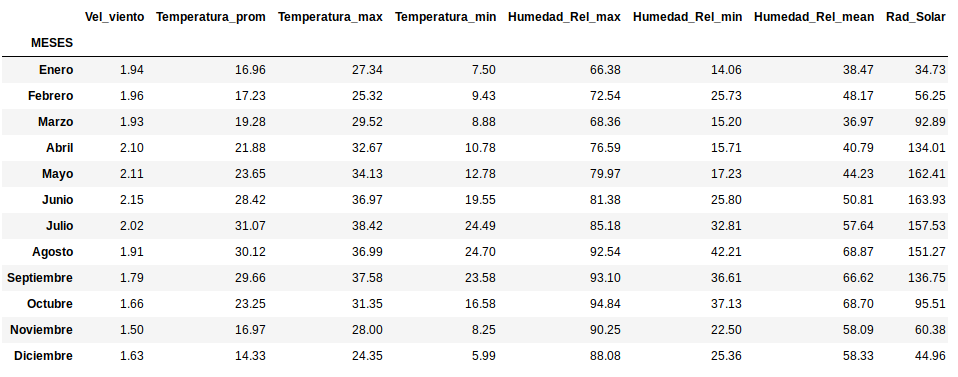
\includegraphics[width=1\textwidth]{tabla_param.png}
\caption{\label{fig:graf1}: Promedios mensuales para un viñedo ubicado en el kilómetro 41 de la carretera de Hermosillo a Bahía Kino (Latitud 28\º 55.117' N, Longitud 111\º 18.638' W, altitud 101m).}
\end{figure}


A partir de esta tabla se realizaron las gráficas para temperatura, humedad relativa y radiación solar mensuales mostradas a continuación.

\begin{figure}[H]
\centering
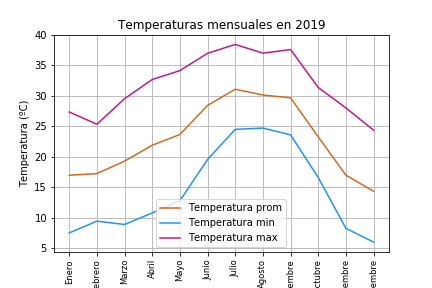
\includegraphics[width=0.7\textwidth]{T_2019.png}
\caption{\label{fig:graf2}: Promedio mensual de temperaturas en 2018.'}
\end{figure}

\begin{figure}[H]
\centering
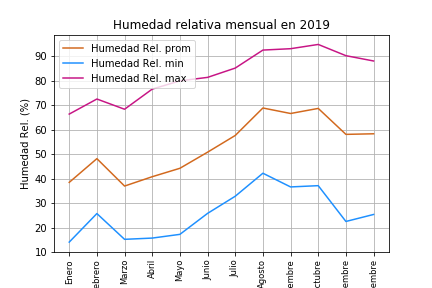
\includegraphics[width=0.7\textwidth]{HR_2019.png}
\caption{\label{fig:graf3}: Promedio mensual de humedad relativa en 2018.}
\end{figure}

\begin{figure}[H]
\centering
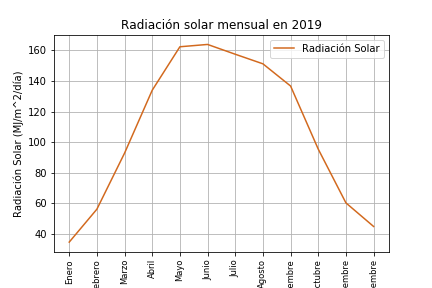
\includegraphics[width=0.7\textwidth]{Rs_2019.png}
\caption{\label{fig:graf1}: Promedio mensual de radiación solar en 2018. }
\end{figure}


\subsubsection{Parte 2}
En esta parte se obtuvo una tabla de comparación para los valores de $ET_{0}$ calculados con tres ecuaciones planteadas por distintos autores.

\begin{figure}[H]
\centering
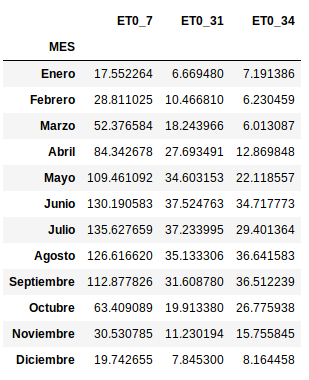
\includegraphics[width=0.5\textwidth]{eto.png}
\caption{\label{fig:graf1}: Estimación de la evapotranspiración de acuerdo a las ecuaciones de Jansen & Haise (Ec.7) y, Valiantzas (Ec. 31 y 34). }
\end{figure}

\subsubsection{Parte 3}
Aquí se obtuvieron gráficas que muestran el balance de energía (energía que entra y sale de la superficie) para un día y para un mes.

\begin{figure}[H]
\centering
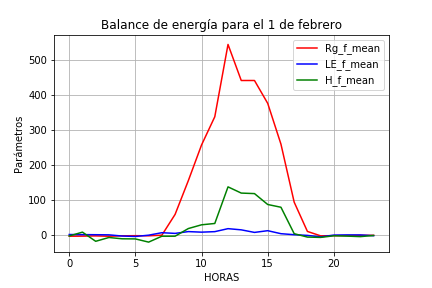
\includegraphics[width=0.5\textwidth]{balance_enero.png}%
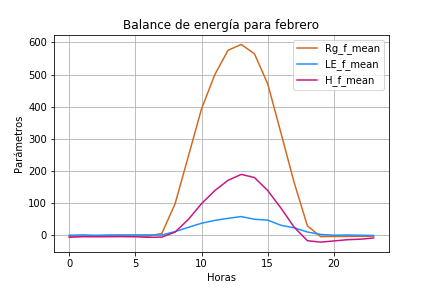
\includegraphics[width=0.5\textwidth]{balance_febrero1.png}
\caption{\label{fig:graf1}: Balance de energía promedio en un día y en un mes.}
\end{figure}
\newpage


\section{Conclusiones}


\section*{Bibliografía}
\begin{itemize}

\item \\Python Strings, Functions and Examples. Recuperado el 8 de abril de 2019 desde \\https://www.techbeamers.com/python-strings-functions-and-examples/
\\

\item \\Merge, join and concatenate. Recuperado el 8 de abril de 2019 desde \\https://pandas.pydata.org/pandas-docs/stable/user\_guide/merging.html
\end{itemize}


\end{document}
